% Section content template for individual Educative lessons
% This file contains the actual content for a specific section
% Generated from Educative API section content

% Section: System Design: Sequencer
% Section ID: 6499939719053312
% Section Slug: system-design-sequencer
% Generated: 2025-12-07T17:28:15.461946

\subsection{Motivation}\label{vckI62tVWabljIodqsUmu}
\\
There can be millions of events happening per second in a large distributed system. Commenting on a post on Facebook, sharing a Tweet, and posting a picture on Instagram are just a few examples of such events. We need a mechanism to distinguish these events from each other. One such mechanism is the assignment of globally unique IDs to each of these events.
\\
Assigning a primary key to an entry in a database is another use case of a unique ID. Usually , the auto-increment feature in databases fulfills this requirement. However, that feature won't work for a distributed database, where different nodes independently generate the identifiers. For this case, we need a unique ID generator that acts as a primary key in a distributed setting---for example, a horizontally-sharded table.
\\
A unique ID helps us identify the flow of an event in the logs and is useful for debugging. A real-world example of unique ID usage is Facebook's end-to-end performance tracing and analysis system, Canopy(An End-to-End Performance Tracing and Analysis System). \textbf{Canopy} uses TraceID to identify an event uniquely across the execution path that may potentially perform hundreds of microservices to fulfill one user request.

\begin{figure}[htbp]
 \centering
 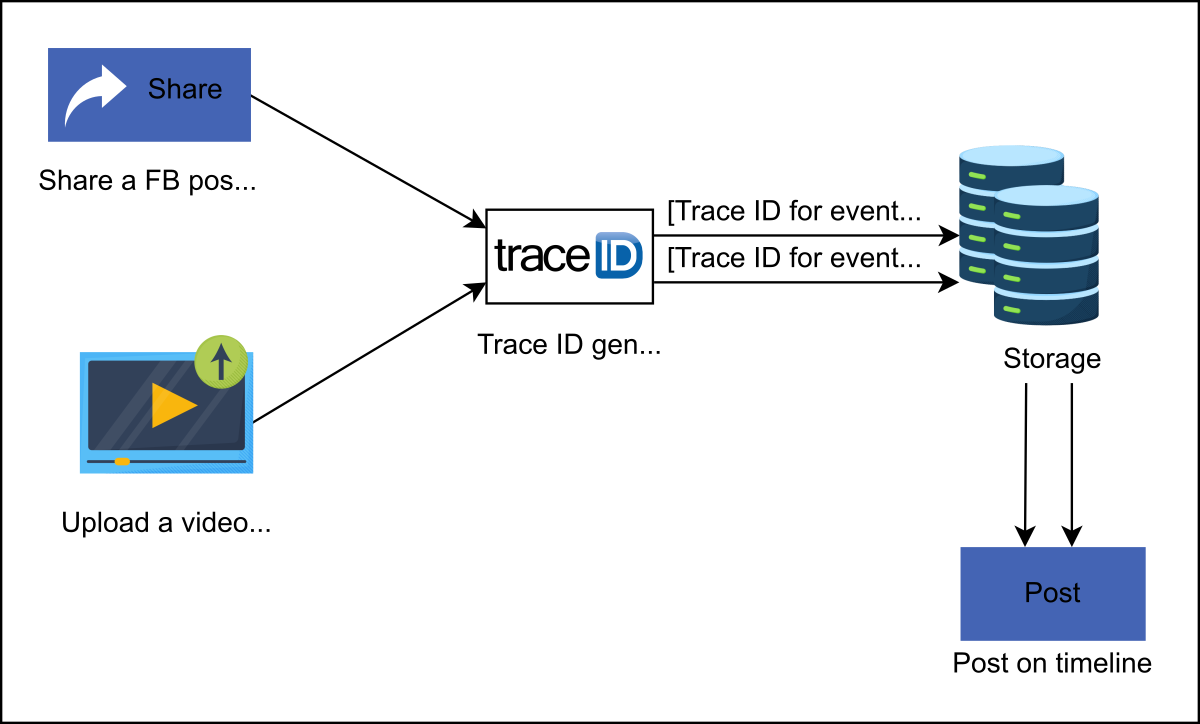
\includegraphics[width=0.5\textwidth]{Images/chapter_12/section_6499939719053312/5359678718869504.png}
 \caption{Assigning a unique TraceID to each event}
\end{figure}

Explain why we need to design a time-sortable unique ID generator.~\\
\\
Use the AI assessment widget below to submit your solution and get an interactive response.

\textbf{Question:}

Why do we prefer time-sortable UIDs?

\textbf{Reference Answer:}

Time-sortable IDs ensure that events or objects are chronologically ordered, which is essential because nearly everything in a system---such as new requests, failures, data creation or deletion, and logs---can be considered an event. Maintaining a time-based order helps in analyzing event sequences, debugging issues, and performing efficient database queries by enabling quick retrieval of the most recent or relevant data.

\subsection{How do we design a sequencer?}\label{XVObYuAQ_XJlsZK-ozI3j}
\\
We've divided the sequencer's comprehensive design into the following two lessons:

\begin{enumerate}
\item
\protect\phantomsection\label{U2eUeXg3Cl28hxBh8ZVS-}
\href{https://www.educative.io/courses/grokking-the-system-design-interview/design-of-a-unique-id-generator}{\textbf{Design of a Unique ID Generator:}} After enlisting the requirements of the design, we discuss three ways to generate unique IDs: using UUID, using a database, and using a range handler.
\item
\protect\phantomsection\label{F-gGB8IE4sdLQNEg9xGYX}
\href{https://www.educative.io/courses/grokking-the-system-design-interview/unique-ids-with-causality}{\textbf{Unique IDs with Causality:}} In this lesson, we incorporate an additional factor of time in the generation of IDs and explain the process by taking causality into consideration.
\end{enumerate}
\\
\textbf{Unique IDs} are important for identifying events and objects within a distributed system. However, designing a unique ID generator within a distributed system is challenging. In the next lesson, let's look at the requirements for a distributed unique ID generation system.

% End of section content